% Chapter Template

\chapter{Distortion Model} % Main chapter title

\label{Chapter3} % Change X to a consecutive number; for referencing this chapter elsewhere, use \ref{ChapterX}

In this chapter we begin by describing how we adapted the preexisting motion retargeting software in order to obtain the desired distorted behavior, and then we detail our distortion model and what function we used. The end of the chapter is dedicated to additional modifications we propose to the work of Molla et al.\ \cite{molla2017egocentric}.

\section{Egocentric Coordinates Distortion}

As briefly mentioned in Chapter \ref{Chapter2}, we are taking advantage of the Egocentric Coordinate formalism in order to introduce our distortion model. We modify each relative displacement vectors $\vec{v}_i$ according to some value $\gamma$. A distorted position $\vec{p}_j$ is thus obtained using equation \ref{eq:DistortionOperation}, which has been obtained by modifying Equation \ref{eq:EgocentricPosition} using a function that we are going to detail in the next few lines.

\begin{equation}
\label{eq:DistortionOperation}
\vec{p}_j = \displaystyle\sum_{i=1}^{n} \hat{\lambda}\big(\vec{x}_i + D(\vec{v}_i,\gamma )\big)
\end{equation}

Figure \ref{fig:armExamples} shows an example of a distorted position obtained by changing the length of all vectors $\vec{v}_i$. This arm model was implemented from the ground up using the FABRIK algorithm as an IK solver \cite{aristidou2011fabrik}. More considerations on this particular implementation can be found in Section \ref{sec:testingApp}.

\begin{figure}[h]
    \centering
    \begin{subfigure}[b]{0.2\textwidth}
        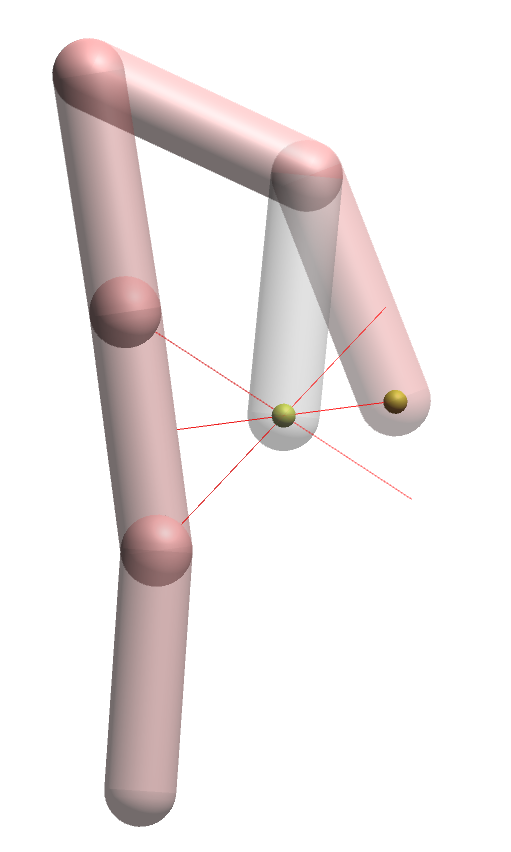
\includegraphics[width=\textwidth]{Figures/simple_distortion_3.png}
        \caption{$\gamma = 3$}
    \end{subfigure}
    ~ %add desired spacing between images, e. g. ~, \quad, \qquad, \hfill etc.
    %(or a blank line to force the subfigure onto a new line)
    \begin{subfigure}[b]{0.2\textwidth}
        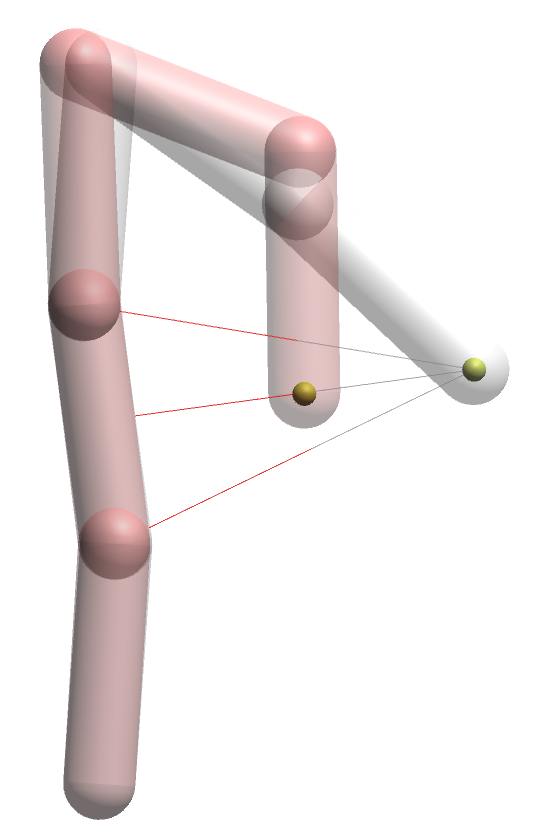
\includegraphics[width=\textwidth]{Figures/simple_distortion_-3.png}
        \caption{$\gamma = -3$}
    \end{subfigure}
    \caption{Two examples of our linear distortion applied to a simple IK arm with multiple segments. The gray lines are the relative displacement vectors and the red ones are their distorted counterparts. Similarly, the gray arms represent the pose the real arm would take whereas the red ones show the two resulting distorted poses.}
    \label{fig:armExamples}
\end{figure}

We will now describe the function we will be using in our subsequent experiment, and then propose a distortion expression that may be better-suited for real-world applications.

\section{Linear Function}
\label{sec:linearFunction}
We are considering candidate functions $D$ to use in Equation \ref{eq:DistortionOperation}. For ease of experimentation and clarity, we are looking for a linear function $f(x) = ax + b$. Figure \ref{fig:armExamples} gives an example of what we aim to achieve, while Figure \ref{fig:plotsOfGamma} below gives a more mathematical point of view of the distortion we are looking for, especially in terms of $a$, the slope of the function. This plot, as well as all of the other plots of this report, were obtained using the Plotly API \cite{plotly}.

\begin{figure}[h]
    \center{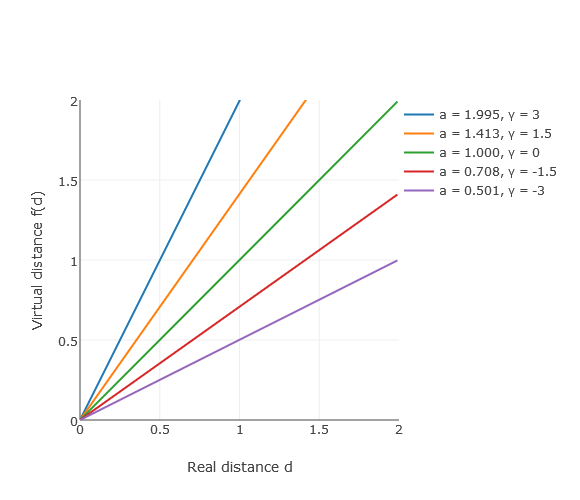
\includegraphics[width=.8\textwidth]
    {Figures/gamma_values.png}}
    \caption{An example of a few distortion functions for various values of slope $a$ and gain $\gamma $.}\label{fig:plotsOfGamma}
\end{figure}

First of all we want to preserve self-haptic contacts. Such contact happens when a relative displacement vector satisfies $\norm{\vec{v}} = 0$, which means that we need $f(0) = 0$, and thus $b = 0$.

Intuitively, the slopes should be arranged around $a=1$, which results in no distortion at all and that we want to correspond to $\gamma = 0$. One can also figure out that there is a correspondence between slopes above and below the line $f(x) = x$. For instance, for a given virtual distance to cover, a slope of \num{0.5} makes the traveling distance twice as long, whereas a slope of \num{2} halves the required movement.

Formally, we are modifying each relative displacement vector as specified in Equation \ref{eq:DistortionOperation}, with $\gamma$ representing a gain, measured in \SI{}{\decibel}, and $f$ defined by Equation \ref{eq:DistortionFunction} below.

\begin{equation}
\label{eq:DistortionFunction}
D(\vec{v},\gamma ) = \hat{\vec{v}} \cdot \norm{\vec{v}} \cdot 10^{\frac{\gamma}{10}}
\end{equation}

In this equation, $\vec{v}$ is a vector, $\hat{\vec{v}}$ is its normalized counterpart, and $\gamma \in \mathbb{R}$. The last factor, $10^{\frac{\gamma}{10}}$, comes from the definition of a gain, in \SI{}{\decibel} \cite{book:decibel}, based on two values $P_1$ and $P_2$ of a single, yet undefined unit:

\begin{align*}
    \text{gain} = \gamma &= 10 \cdot \log_{10} (\frac{P_1}{P_2})\\
    \frac{\gamma}{10} &= \log_{10} (\text{slope})\\
    \text{slope} &= 10^{\frac{\gamma}{10}}.
\end{align*}

A value of $\gamma = 3$ thus indicates that the virtual movement will roughly be twice the amplitude of the registered one ($1.995 \approx 2$), while a gain of $\gamma = -3$ means one will have to travel twice as big a distance (\num{0.501}) as perceived in order to cover it. Figure \ref{fig:armExamples} shows two examples of distortion, and Figure \ref{fig:plotsOfGamma} gives a few instances of this linear distortion functions with varying values of $\gamma $ and the corresponding slope $a$.

\section{Other Functions}
\label{sec:otherFunctions}
Before deciding to use a simpler, thus easier to quantify, linear function for our experimentation process, we tried out different functions that we think are of interest for further applications. Two of these functions are described here as a reference for further investigation.

As for our linear function, we require the distortion to be null around $\norm{\vec{v}} = 0$. Similarly, we introduce an action range $a_r$ after which the distortion should be null again. The general form of the function applied to our relative displacement vectors then becomes the one described in Equation \ref{eq:distortionCase}.

\begin{equation}
    \label{eq:distortionCase}
    D(\vec{v}, s, a_r) =
    \begin{cases}
        \hat{\vec{v}} ~ f(\norm{\vec{v}}, s, a_r)    &\text{if } \norm{\vec{v}} \leq a_r\\
        \vec{v}                                                         &\text{otherwise}
    \end{cases}
\end{equation}

Note that we changed the `$\gamma $' parameter for `$s$', which is due to this parameter no longer denoting a cleanly defined gain, but a vaguer concept of strength. Two notable instances of the function $f$ were implemented. They are shown in Figure \ref{fig:otherDistortions} and are described hereafter.

\begin{figure}[h]
    \centering
    \begin{subfigure}[b]{.45\textwidth}
        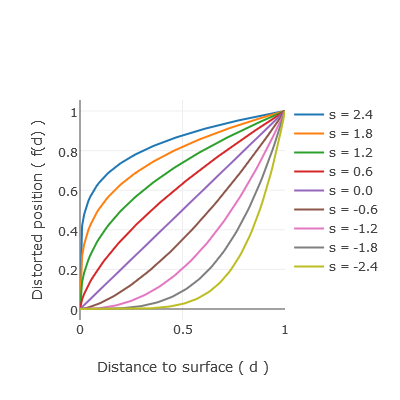
\includegraphics[width=\textwidth]{Figures/exponential_distortion.png}
        \caption{Exponential}
        \label{fig:otherDistortionsExp}
    \end{subfigure}
    ~
    \begin{subfigure}[b]{.45\textwidth}
        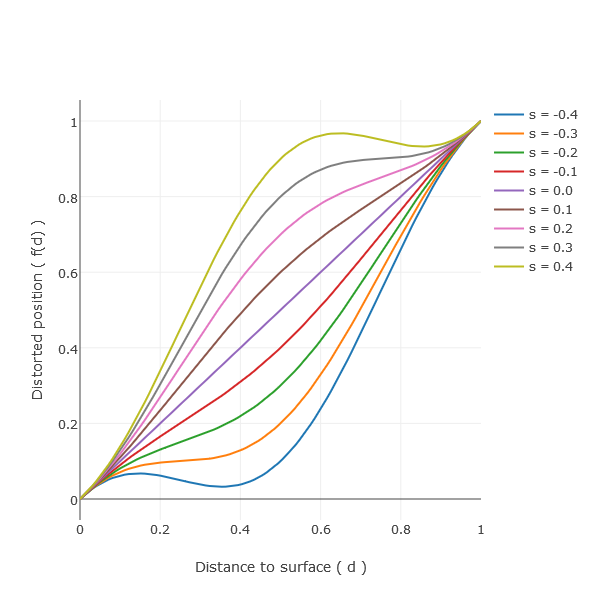
\includegraphics[width=\textwidth]{Figures/cosine_distortion.png}
        \caption{Cosine}
        \label{fig:otherDistortionsCos}
    \end{subfigure}
    \caption{Multiple instances of the two alternative distortion functions we propose in section \ref{sec:otherFunctions}. Both have been plotted using $a_r = 1$, only varying the strength parameter $s$.}
    \label{fig:otherDistortions}
\end{figure}

\subsection*{Exponential}

Based on an expression proposed by Khoury \cite{khoury2015human}, this function has the following form:

\begin{equation*}
    f(d, a_r, s) = a_r \cdot \Bigg(\frac{d}{a_r}\Bigg)^{2^{-s}}
\end{equation*}

As one can observe on Figure \ref{fig:otherDistortions}, this function has the advantage of smoothly transitioning from a non-distorted position to a maximum discrepancy, and then back to an undistorted position near $d=a_r$. This behavior however comes at a cost. At high strength values (e.g.\ $s=2.4$) we observe a severe jump in position when the hand departs from the skin: in a few centimeters in the real world, the virtual hand already jumps to almost two thirds of the action range. For equally high negative values the behavior is similar in that the hand seems to `wait' on the skin for a long while before speeding up to rejoin the hand and approaching the other end of the action range. This high velocity discrepancy gets easily noticed and further investigations should be made as per what strength is acceptable.

\subsection*{Cosine}

Observations made on the previous function led us to designing this second function, that is smoother in terms of velocity discrepancy near the ends of the range of the function. It is defined as:

\begin{equation*}
    f(d, a_r, s) = \frac{s}{2}\Bigg(1 - \cos\Big(\frac{2\pi}{a_r} \cdot d\Big)\Bigg) + d
\end{equation*}

Obviously, being smoother in terms of velocity near both ends of the distorted area leads to trade-offs. In our case the function introduces higher velocity discrepancies at other locations, as one can observe on Figure \ref{fig:otherDistortionsCos}. At high strengths (e.g.\ $s=0.4$) the function even forces the virtual hand to go backwards in order to rejoin the real position before approaching $a_r$.

Again, both of these functions are an attempt at fixing the behavior of the distortion when going further away from the skin, but further experimentation is needed in order to determine how they affect both our acceptation of a distorted movement as our own, and the SoE through their respective effects on the Sense of Agency.

\section{Egocentric Normalization Factor}

We added one more modification to the definition of the position proposed by \cite{molla2017egocentric} which we modified to obtain Equation \ref{eq:DistortionOperation}, and more precisely the way $\lambda $ is defined. As originally explained by \cite{molla2016precise} as well as in Section \ref{sec:egocentric}, it is computed as the product of two importance factors, proximity and orthogonality, respectively denoted $\lambda_p$ and $\lambda_\perp $.

The former importance factor was initially defined as $\lambda_p = \frac{1}{\norm{\vec{v}}}$. In practice we find that this formula does not give enough importance to nearby body parts, and we decided to change it slightly as $\lambda_p = \frac{1}{\norm{\vec{v}}^2}$, thus becoming proportional to the inverse square of the distance between the surface and the point. We find this definition elegant since it matches the form of an inverse square law (such as Coulomb's law, or Netwton's law of universal gravitation), of the form:

\begin{equation*}
    \text{intensity} \propto \frac{1}{\text{distance}^2}
\end{equation*}

This indeed has a physical justification: a point-source geometrically dilutes its radiated energy, force, or any other conserved quantity in three-dimensional space, hence the influence of the inverse square of the distance between that point-source and a given surface. In our case we can consider the ``amount of distortion'' received by any point in space in a similar way. Moreover, this gives more consistent practical results in the sense that when moving the hand horizontally in front of the torso, that hand is less affected by other body parts such as the legs or the head.

\section{Reachable Sphere}
\label{sec:reachableSphere}

Molla et al. \cite{molla2017egocentric} proposed a special case for handling the position of the feet: they use the orthogonal projection of the ankle on the floor as an additional reference point, hence adding one Egocentric component to the coordinates of that joint.

\begin{figure}[h]
    \centering
    \begin{subfigure}[b]{.35\textwidth}
        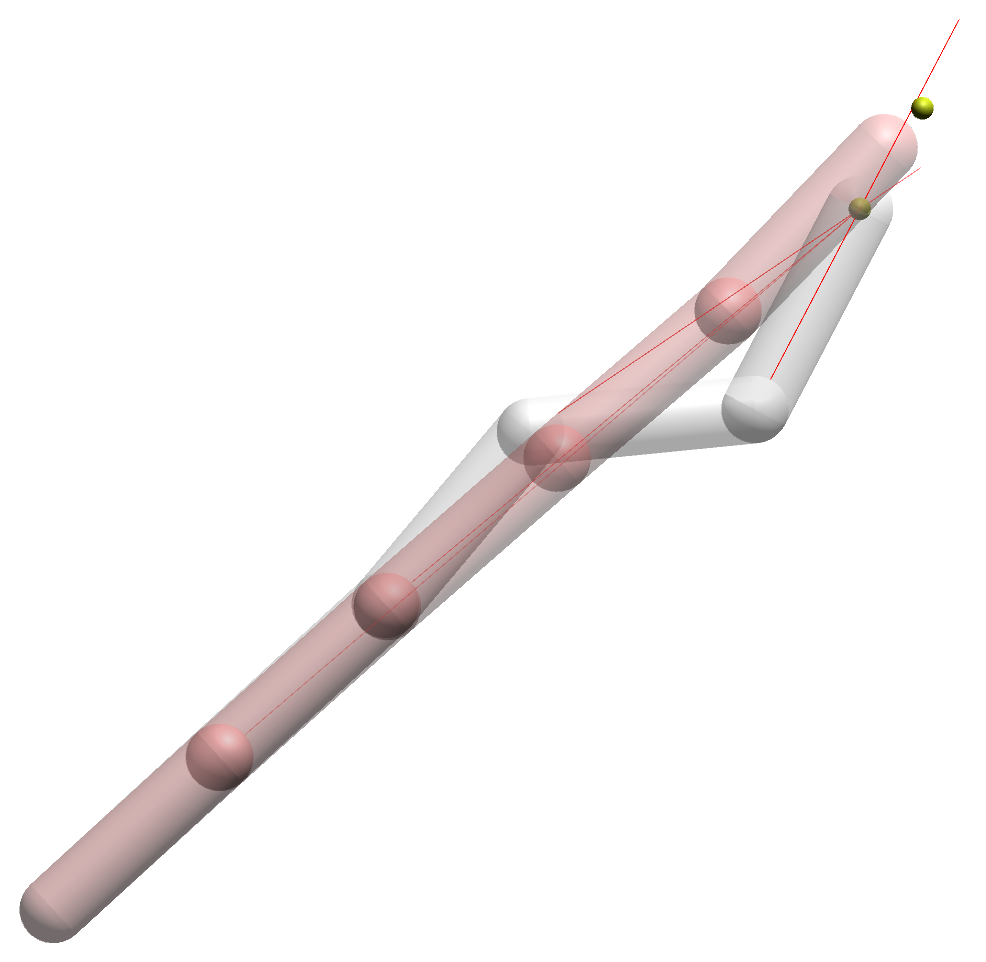
\includegraphics[width=\textwidth]{Figures/arm-full-nosphere.png}
    \end{subfigure}
    ~
    \begin{subfigure}[b]{.35\textwidth}
        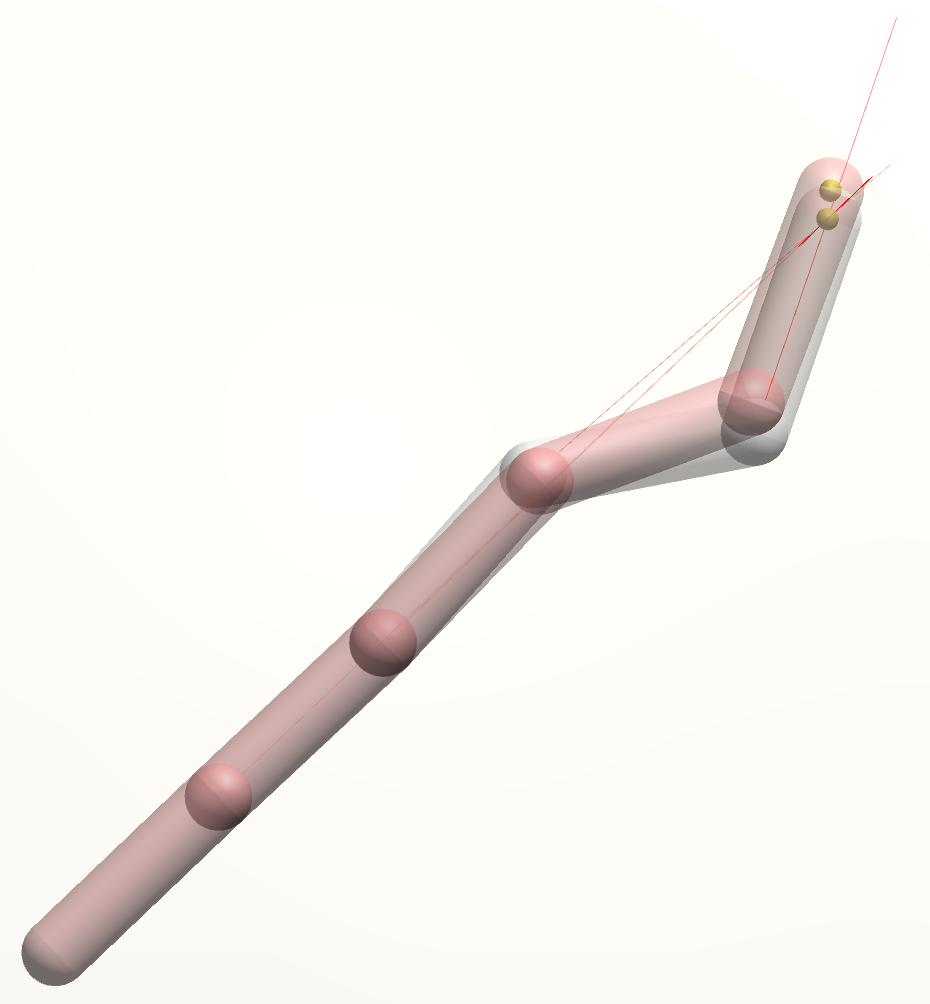
\includegraphics[width=\textwidth]{Figures/arm-full-sphere.png}
    \end{subfigure}
    \label{fig:fullSphere}
    
    \vspace{1em}
    
    \begin{subfigure}[b]{.24\textwidth}
        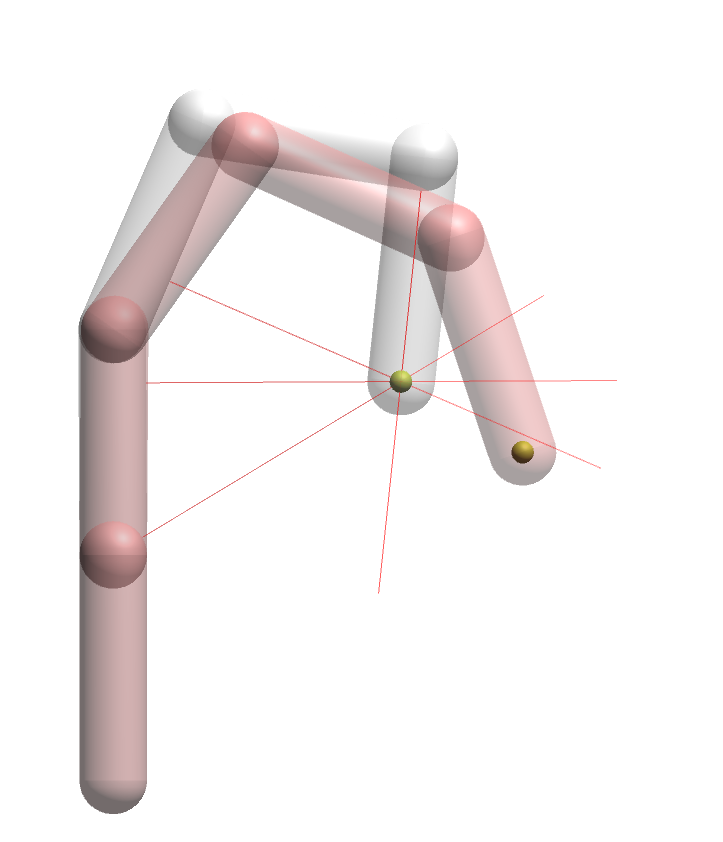
\includegraphics[width=\textwidth]{Figures/arm-mid-nosphere.png}
    \end{subfigure}
    \hspace{4em}
    \begin{subfigure}[b]{.35\textwidth}
        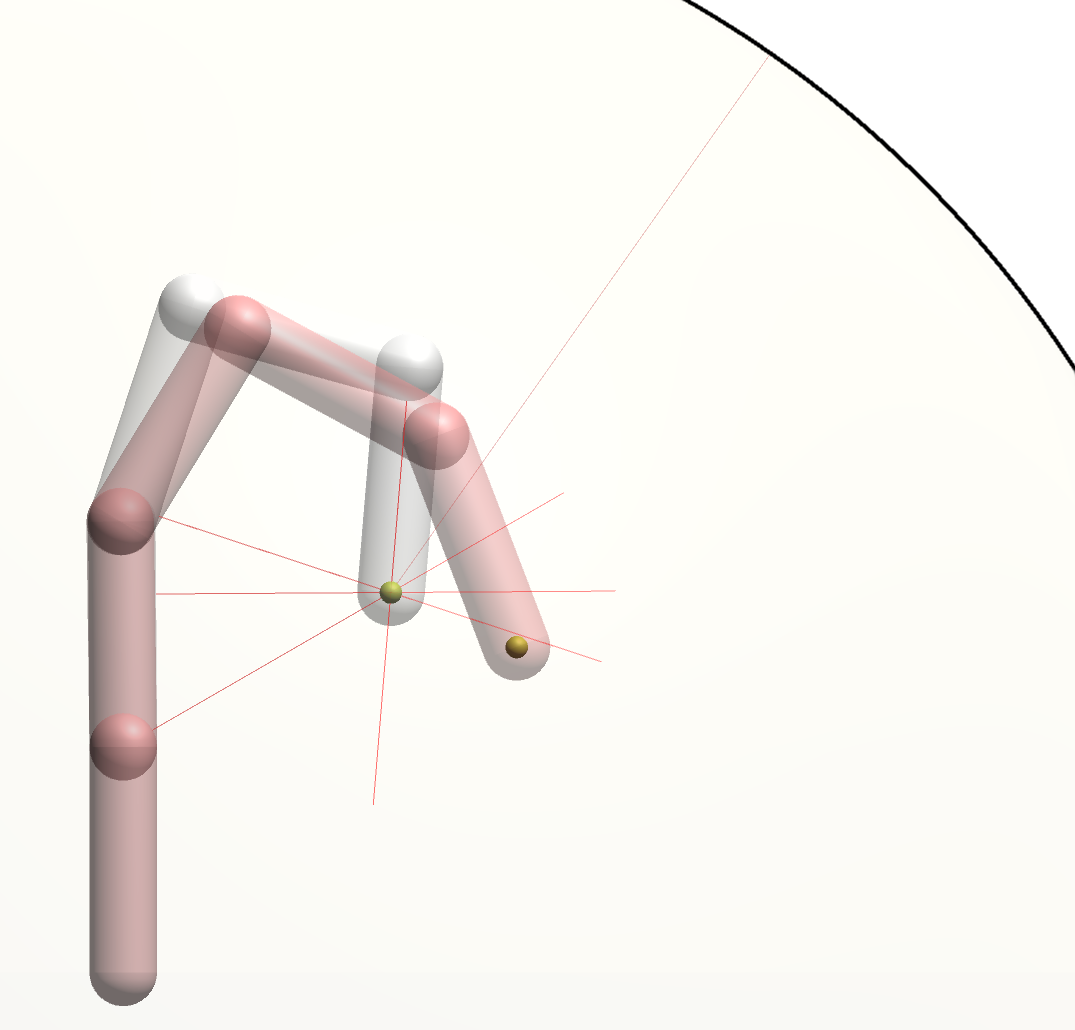
\includegraphics[width=\textwidth]{Figures/arm-mid-sphere.png}
    \end{subfigure}
        
    \caption{An example of undesired pose behavior near full arm extension (top left) and how we propose to solve it (top right) using the reachable sphere, in light yellow and outlined on the top right corner for readability. A pose far from the surface of the sphere is almost not affected (bottom left and right). The captured arms are in gray, the distorted ones in red, and the red lines represent the distorted coordinates.}
    \label{fig:reachableSphere}
\end{figure}

We think that interactions close to the far end of the reachable volume of each arm may benefit from such an additional reference point as well, especially when considering distortions made to the wrist position. To do so, we propose the addition of a sphere of radius equal to the arm's length and centered on the shoulder of that arm, that we call ``reachable sphere''. When approaching full arm extension, the position of the wrist relative to that reachable sphere becomes prominent and forces to distortion to act as if the hand was approaching one's skin: it would tend towards a null distortion. Figure \ref{fig:reachableSphere} illustrate the type of pose behavior we attempt to avoid by introducing this reachable sphere, as well as shows that it does almost not affect movements closer to other body parts.

In the experiment described in Chapter \ref{Chapter4} we however did not implement this reachable sphere for two reasons. First, it greatly alters the linear nature of the distortion function we proposed in Section \ref{sec:linearFunction} and thus is not desired in such an experimental context. The second reason is more practical: the retargeting software is quite complex and unfortunately poorly commented, which makes such a modification very hard to achieve.

\section{Testing Application}
\label{sec:testingApp}
The simple kinematic chain we used for preliminary testing and to obtain for instance Figure \ref{fig:armExamples} was built using the description of the Egocentric Formalism provided by \cite{molla2016precise}. For ease of use, we integrated a preexisting IK solver to this implementation, namely the FABRIK algorithm proposed by Aristidou and Lasenby \cite{aristidou2011fabrik}. We encountered one issue when using this testing application once the distortion was implemented: depending on the sequence of movements of the IK goal, the actual kinematic chain and the distorted one began to have diverging intermediary joint positions, such as shown in Figure \ref{fig:divergence}.

\begin{figure}[h]
    \centering
    \begin{subfigure}[b]{0.22\textwidth}
        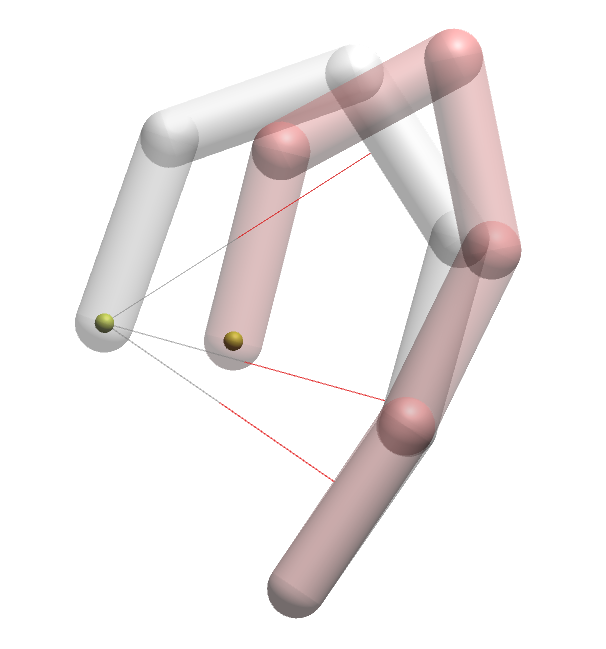
\includegraphics[width=\textwidth]{Figures/arm_noDivergence.png}
        \caption{Initial pose.}
        \label{subfig:divergenceInitial}
    \end{subfigure}
    ~
    \begin{subfigure}[b]{0.3\textwidth}
        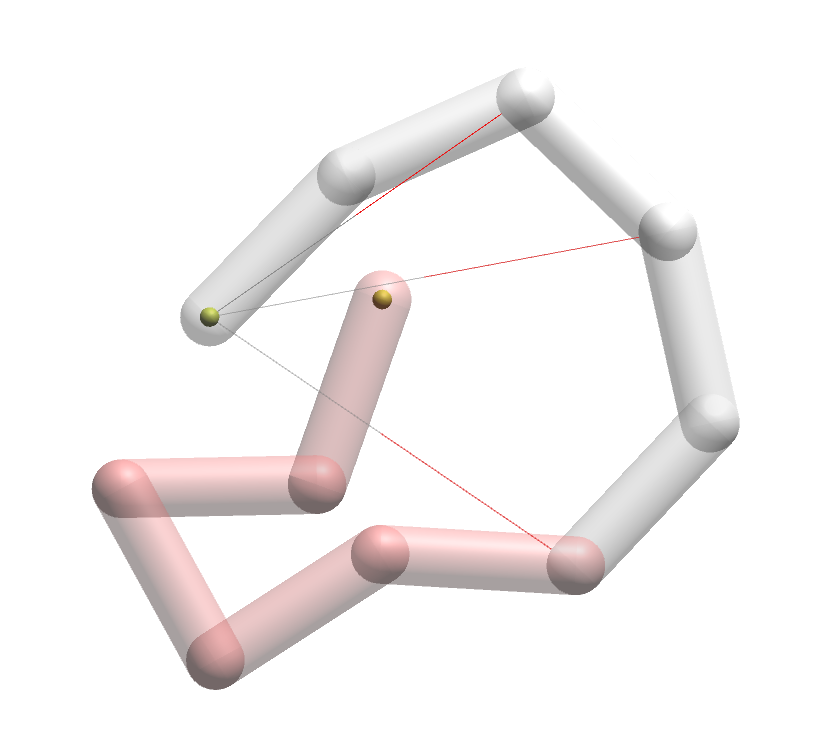
\includegraphics[width=\textwidth]{Figures/arm_divergence.png}
        \caption{Diverging poses.}
        \label{subfig:divergence}
    \end{subfigure}
    ~
    \begin{subfigure}[b]{0.3\textwidth}
        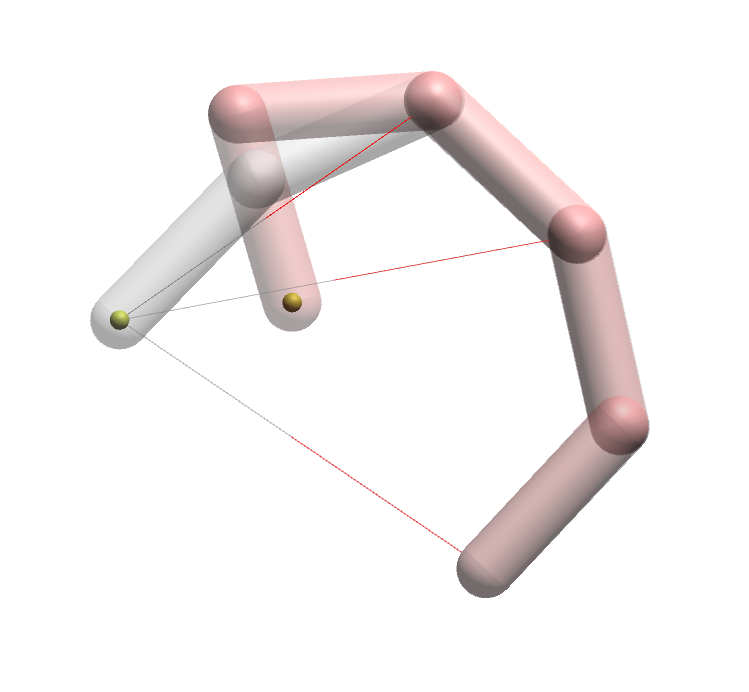
\includegraphics[width=\textwidth]{Figures/arm_initDivergence.png}
        \caption{With pose re-initialization.}
        \label{subfig:initDivergence}
    \end{subfigure}
    \caption{In gray are the real arms whose movements are supposedly captured through their respective IK goals (yellow spheres inside the last capsule), and in red are the distorted poses, which are the ones a end user would see in the virtual environment. An example of initial IK chains (left) and the diverging poses after a certain sequence of movements (center). The pose can then be corrected by initializing the distorted arm at the real arm's position (right).}
    \label{fig:divergence}
\end{figure}

Two options exist in order to solve this issue. The first one is to introduce secondary IK goals at what can be considered as the `ellbows' of the arm. The second option is to re-initialize the distorted arm at the real arm pose before running the IK iterations. While we chose the latter for our testing application, the former is probably better-suited for real world applications, where markers are available all over the body and may serve to determine such secondary IK goal.